\documentclass{beamer}



\usepackage[utf8]{inputenc}
\usepackage[ngerman]{babel}
\usepackage{verbatim}
\usepackage{hyperref}
\usepackage{url}
\usepackage{fancyvrb}

\title{JOSM Workshop}
\author{Stefan Tiran  osm@stefantiran.at}
\date{April 27th, 2018}

\usetheme{Antibes}

%\usebackgroundtemplatei{
%\includegraphics[width=\paperwidth,
%height=0.8\paperheight]{mag_map.png}
%}

\begin{document}

%\maketitle

%\begin{frame}


%\begin{figure}
%  \centering
%  \includegraphics[angle=90,width=.3\textwidth]{IMG_6589.JPG}
%\end{figure}

%\begin{center}
%\Large{Anwendung von freien Geodaten auf mobilen Navigationsgeräten\\}
%\end{center}

%\begin{center}
%{\emph{Freie Karten, Routen und POIs auf herkömmlichen Navigationsgeräten verwenden}}
%\end{center}
%\end{frame}

\begin{frame}{Agenda}
  \begin{itemize}
    \item Erste Demo zum Kennenlernen
    \item Vorstellung des Vortragenden
    \item Kurze Einführung in das OSM--Datenmodell
    \item Kurzer Überblick über das OSM--Wiki
    \item Eingabe von Adressen
    \item Arbeiten mit Layern
    \item Arbeiten mit unterschiedlichen Datenformaten

  \end{itemize}
\end{frame}

\begin{frame}{Über den Vortragenden}

  \begin{itemize}
    \item Stefan Tiran \textless \href{mailto:osm@stefantiran.at}{osm@stefantiran.at}\textgreater
    \item IT--Entwickler an der Universität Wien
    \item Linux-User (SuSE / Ubuntu) seit 2003
    \item OpenStreetMap seit August 2008
    \begin{itemize}
      \item OSM-Username: \emph{StefanTiran}
      \item Mapping-Area: Marchfeld, Graz, Südsteiermark
    \end{itemize}
  \end{itemize}
\end{frame}

\begin{frame}[fragile]{Das OpenStreetMap--Datenmodell}

Das OSM-Datenmodell besteht aus den folgenden Elementen:
\begin{itemize}
  \item 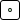
\includegraphics[height=0.8em]{node}\hspace{0.2em} Punkt bzw. Knoten (englisch: node) 
  \item 
\includegraphics[height=0.8em]{way} \hspace{0.2em} 
\includegraphics[height=0.8em]{closed_way}\hspace{0.2em} Linie (englisch: way)
  \item 
\includegraphics[height=0.8em]{area} \hspace{0.2em} Fläche (english: area) 
  \item 
\includegraphics[height=0.8em]{relation} \hspace{0.2em} Relation (english: relation) 
  \item 
\includegraphics[height=0.8em]{tag} \hspace{0.2em}Attribut (english: tag) 

\end{itemize}

Quelle: \url{https://wiki.openstreetmap.org/wiki/DE:Elemente}

\end{frame}

\begin{frame}[fragile]{Punkt}

\begin{itemize}
  \item auch Knoten (englisch: node)
  \item Georeferenzierter Punkt mit Längen- und Breitengrad
  \item kann Eigenschaften (Attribute) haben
  \item kann Teil eines Weges (einer Linie) sein
  \item kann Teil einer Relation sein
\end{itemize}

Quelle: \url{https://wiki.openstreetmap.org/wiki/DE:Node}

\end{frame}

\begin{frame}[fragile]{Linie}
\begin{itemize}
  \item auch Weg (englisch: way)
  \item Sequenz von 2 - 2000 Punkten
  \item kann Punkte auch mehrfach enthalten
  \item kann dadurch offenen oder geschlossenen Linienzug darstellen
  \item hat eine Richtung
\end{itemize}

Quelle: \url{https://wiki.openstreetmap.org/wiki/DE:Way}

\end{frame}
\begin{frame}[fragile]{Fläche}

\begin{itemize}
  \item auch Fläche, Gebiet oder ausgefülltes Polygon
  \item kein eigentständiges Element im Datenmodell
  \item Modellierung als geschlossene Linie
  \begin{itemize}
    \item entweder explizit durch \texttt{area=yes} oder implizit
  \end{itemize}
  \item Modellierung als Polygon
  \begin{itemize}
    \item Typ: Multipolygon (\texttt{type=multipolygone})
  \end{itemize}
\end{itemize}
Quelle: \url{https://wiki.openstreetmap.org/wiki/DE:Area}
\end{frame}
\begin{frame}{Relation}
\begin{itemize}
  \item sortierte Liste von Datenelementen
  \item jedem Datenelement kann eine Rolle zugewiesen werden
  \item Beispiel-Typen
  \begin{itemize}
    \item Route (\texttt{type=route})
    \item Multipolygon (\texttt{type=multipolygone})
    \item Abbiegebeschränkung (\texttt{type=restriction})
   \end{itemize}
\end{itemize}
Quelle: \url{https://wiki.openstreetmap.org/wiki/DE:Relationen}
\end{frame}

\begin{frame}
Folien zum JOSM--Workshop auf den
\href{http://http://linuxtage.at/}{Grazer Linuxtagen} am 27. 4. 2018.
\vspace{1cm}

Folien unter 
\includegraphics[width=1cm]{cc-by-sa.png}.
\vspace{1cm}

Erstellt mittels \LaTeX Beamer, Source auf \url{https://github.com/StefanTiran/josm_ws_glt18/}.
\vspace{1cm}

\href{mailto:osm@stefantiran.at}{Stefan Tiran}
\end{frame}


\end{document}


%%:foldmethod=expr
%% vim:fde=getline(v\:lnum)=~'^%%%%\ .\\+'?'>1'\:'='
%%% Local Variables: 
%%% mode: latex
%%% mode: auto-fill
%%% mode: flyspell
%%% eval: (ispell-change-dictionary "de_AT")
%%% TeX-master: "main"
%%% End: 

